\documentclass{article}

\usepackage[utf8]{inputenc}
\usepackage[T1]{fontenc}
\usepackage{hyperref}
\usepackage{tabularx}
\usepackage{array}
\usepackage{fancyhdr}
\usepackage{graphicx}
\usepackage[a4paper]{geometry}
\usepackage{multicol}
\usepackage{listings}
\usepackage{pgfplots}

\pgfplotsset{width=10cm,compat=1.9}

\title{Apprentissage automatique \\ Le jeu de Nim}
\author{par Camille Leplumey et Geoffrey Spaur}
\date{03 Mai 2017}
\pagestyle{fancy}
\lhead{Apprentissage automatique - Le jeu de Nim \\ \textbf{M1GIL} - Camille Leplumey et Geoffrey Spaur}
\rhead{
\includegraphics[scale=0.5]{logo_univ_rouen.png}}
\setlength{\headsep}{1cm}
\begin{document}

\maketitle
\newpage
\tableofcontents{}
\newpage
\section{Mode \emph{easy}}
  \paragraph{}
    Le CPU joue aléatoirement sans prendre de décisions. Il est donc possible qu'il perde bêtement. 
    Le CPU jouera entre 1 et 3 bâtons comme indiqué dans les règles du jeu.
    Il lui sera cependant interdit de jouer 3 bâton alors qu'il en reste 2. Ainsi il jouera automatiquement 1 bâton, s'il reste 1 bâton en jeu.
    Il jouera, avec 50\% de chance, 1 ou 2 bâtons quand il restera 2 bâtons en jeu.
\section{Mode \emph{medium}}
  \paragraph{}
    Le mode medium ne constitue en rien à de l'apprentissage. En effet nous codons les derniers coups que doit
    jouer le CPU. Le résultat sera donc identique à chaque partie sur les derniers coups et aléatoire sur les autres coups.
  \paragraph{}
    Dans notre cas le CPU jouera:
    \begin{itemize}
     \item 3 s'il reste 4 bâtons
     \item 2 s'il reste 3 bâtons
     \item 1 s'il reste 2 bâtons
    \end{itemize}
    Hormis ces 3 cas spécifiques, le CPU jouera aléatoirement. Il est évident que le CPU jouera 1 s'il reste 1 bâton au même titre que dans le mode \emph{easy}.
    
\newpage
\section{Mode \emph{hard}}
  \paragraph{}
    Ici en entraînant le CPU contre lui-même en mode \emph{hard}, il va apprendre la stratégie gagnante par lui-même sans aide extérieur. 
    C'est un apprentissage \textbf{non supervisé}. Nous utilisons cette méthode car nous pouvons l'automatiser facilement.
  
  \subsection{Protocole des réalisations des graphiques}
  \paragraph{}
    Nous avons réalisé quelques statistiques concernant les différentes façons de jouer.
    Chaque point des courbes est une moyenne de 50 parties jouées. Chaque partie comprend une phase d'apprentissage,
    où le réseau de neurones se construira. Nous avons donc échelonné cette phase d'apprentissage pour réaliser nos graphiques.
    Le CPU apprendra donc sur 100 parties, nous effectuerons cet apprentissage 50 fois afin d'établir une moyenne de réussite.
    Nous procéderons de manière identique avec une phase d'apprentissage à 1.000 parties et ainsi de suite jusqu'à arriver à une phase d'apprentissage à 100.000 parties.
  \paragraph{}
    Il est important de remarquer que notre échelonnage est \textbf{non proportionnel}. Il est donc possible de voir
    des légers paliers sur les différentes courbes des graphiques.
  
  \subsection{Graphique de réussite}
  \paragraph{}
    \begin{tikzpicture}
     \begin{axis}[
	title={Évolution du taux moyen de réussite entre 2 joueurs \textbf{hard} sans changement de rôle},
	ylabel={Taux de réussite en pourcentage },
	xlabel={Nombre de parties},
	ymin=0, ymax=100,ytick={0,20,40,60,80,100},
	xmin=0, xmax=7,xtick={0,1,2,3,4,5,6,7},
	xticklabels={0,100,500,1.000,5.000,10.000,50.000,100.000},
	scaled ticks=false,
	tick label style={/pgf/number format/fixed}, smooth,
	legend entries={Premier joueur,Second joueur},
	legend style={at={(0,1)},anchor=north west},
	legend cell align={left}
    ]
    
    \addplot[color=blue,mark=square,]
	coordinates {(0,50)(1,53)(2,58)(3, 66)(4, 80)(5, 89)(6, 94)(7, 97)};
    \addplot[color=gray,mark=square,]
	coordinates {(0,50)(1,48)(2, 42)(3, 34)(4, 20)(5, 11)(6, 6)(7, 3)};
  
    \end{axis}
    \end{tikzpicture}\\
    Nous voyons ici qu'en jouant 800 parties, le CPU obtiendrai une moyenne de 63\% de réussite. De
    plus, nous pouvons affirmer qu'à partir de 50.000 parties jouées, le CPU ne fera quasiment plus d'erreurs.\\
    
  \subsection{Statistiques selon le mode de joueur}
  \paragraph{}
    \begin{tikzpicture}
     \begin{axis}[
	title={Évolution du taux moyen de réussite d'un joueur \textbf{easy} sans changement de rôle},
	ylabel={Taux de réussite en pourcentage },
	xlabel={Nombre de parties},
	ymin=0, ymax=100,ytick={0,20,40,60,80,100},
	xmin=0, xmax=7,xtick={0,1,2,3,4,5,6,7},
	xticklabels={0,100,500,1.000,5.000,10.000,50.000,100.000},
	scaled ticks=false,
	tick label style={/pgf/number format/fixed}, smooth,
	legend entries={Second joueur easy,Second joueur medium,Second joueur hard},
	legend style={at={(0,1)},anchor=north west},
	legend cell align={left}
    ]
    \addplot[color=green,mark=square,]
	coordinates {(0,49)(1,49)(2, 51)(3, 50.5)(4, 50)(5, 50)(6, 50)(7, 50)};
    \addplot[color=blue,mark=square,]
	coordinates {(0,17)(1,16)(2, 17.5)(3, 17)(4, 17)(5, 17)(6, 17)(7, 17)};
    \addplot[color=red,mark=square,]
	coordinates {(0,50)(1,27)(2, 21)(3, 20)(4, 17)(5, 16)(6, 14)(7, 14)};
  
    \end{axis}
    \end{tikzpicture}
    
  \paragraph{}
    \begin{tikzpicture}
     \begin{axis}[
	title={Évolution du taux moyen de réussite d'un joueur \textbf{medium} sans changement de rôle},
	ylabel={Taux de réussite en pourcentage },
	xlabel={Nombre de parties},
	ymin=0, ymax=100,ytick={0,20,40,60,80,100},
	xmin=0, xmax=7,xtick={0,1,2,3,4,5,6,7},
	xticklabels={0,100,500,1.000,5.000,10.000,50.000,100.000},
	scaled ticks=false,
	tick label style={/pgf/number format/fixed}, smooth,
	legend entries={Second joueur easy,Second joueur medium,Second joueur hard},
	legend style={at={(0,0)},anchor=south west},
	legend cell align={left}
    ]
    \addplot[color=green,mark=square,]
	coordinates {(0,80)(1,81)(2, 81)(3, 82)(4, 81)(5, 81)(6, 81)(7, 81)};
    \addplot[color=blue,mark=square,]
	coordinates {(0,51)(1,51)(2, 49.5)(3, 50)(4, 50)(5, 50)(6, 50)(7, 50)};
    \addplot[color=red,mark=square,]
	coordinates {(0,95)(1,47)(2, 28)(3, 23)(4, 17)(5, 16)(6, 16)(7, 15)};
  
    \end{axis}
    \end{tikzpicture}
  \paragraph{}
    Sans surprise sur ces graphiques, nous ne voyons aucune évolution du taux de réussite contre les joueurs \emph{easy} et \emph{medium}, 
    car ces joueurs ne changent pas leur stratégie au cours du temps.
    Nous pouvons cependant constater de légères variations dans les premières parties dû à un affinement de la moyenne.\\
    Il est à noter que le joueur \emph{hard} apprend plus vite en commeçant en second contre un joueur \emph{easy} que contre un joueur \emph{medium}.
    Cela souligne les différentes façons de jouer des joueurs \emph{easy} et \emph{medium}. Pour rappel le joueur \emph{medium} joue aléatoirement tout comme 
    le joueur \emph{easy}, sauf pour le dernier coup, où le joueur \emph{medium} tentera de gagner.
  
  \paragraph{}
    \begin{tikzpicture}
     \begin{axis}[
	title={Évolution du taux moyen de réussite d'un joueur \textbf{hard} sans changement de rôle},
	ylabel={Taux de réussite en pourcentage },
	xlabel={Nombre de parties},
	ymin=0, ymax=100,ytick={0,20,40,60,80,100},
	xmin=0, xmax=7,xtick={0,1,2,3,4,5,6,7},
	xticklabels={0,100,500,1.000,5.000,10.000,50.000,100.000},
	scaled ticks=false,
	tick label style={/pgf/number format/fixed}, smooth,
	legend entries={Second joueur easy,Second joueur medium,Second joueur hard},
	legend style={at={(1,0)},anchor=south east},
	legend cell align={left}
    ]
    \addplot[color=green,mark=square,]
	coordinates {(0,50)(1,74)(2, 80)(3, 84)(4, 86)(5, 86)(6, 88)(7, 91)};
    \addplot[color=blue,mark=square,]
	coordinates {(0,5)(1,54)(2, 75)(3, 80)(4, 87)(5, 87)(6, 88)(7, 90)};
    \addplot[color=red,mark=square,]
	coordinates {(0,50)(1,53)(2,58)(3, 66)(4, 80)(5, 89)(6, 94)(7, 97)};
  
    \end{axis}
    \end{tikzpicture}\\
    De loin le schéma le plus intéressant. En effet dans la phase 100 à 10.000 parties, nous pouvons voir que le joueur \emph{hard} commençant en premier, à un plus haut taux de réussite 
    contre un joueur \emph{medium}, que contre un second joueur \emph{hard}.
    Cela s'explique par le fait que le joueur \emph{medium} joue aléatoirement alors que le second joueur \emph{hard}
    essaye de découvrir la stratégie gagnante, tout comme le premier joueur \emph{hard}. Le premier joueur \emph{hard}, à partir des 10.000 parties
    perfectionne tellement son réseau que le second joueur \emph{hard} ne peut plus apprendre car il enchaînera les défaites.\\
    Il n'est donc pas surprenant de voir le taux de réussite contre un joueur \emph{medium} dépasser le taux de réussite contre un joueur \emph{hard} car 
    le joueur \emph{medium} ne peut pas se tromper sur le dernier coup contrairement au second joueur \emph{hard}.

  \subsection{Conclusion}
  \paragraph{}
    Pour conclure, si nous voulons jouer contre le CPU en mode \emph{hard}, il sera toujours possible de gagner.
    En effet le CPU choisit aléatoirement parmi ses connexions en favorisant les connexions à fort poids. 
    Néanmoins la chance que le CPU choisisse une connexion perdante sera toujours non nul, car les poids initiaux des connexions sont non nul et ne décroissent jamais. 
    Même si le CPU est bien entraîné, avec de la patience, il sera toujours possible de gagner une partie contre lui.


\newpage

\section{Correction apportée}
  \paragraph{}
    Suite à nos différent tests, nous avons généré et testé un réseau entraîné à jouer en second contre un CPU \emph{medium}.
    Durant notre phase de test, nous avons importé son réseau afin de jouer contre lui (en le plaçant dans le même rôle, c'est-à-dire qu'il va jouer en second).
    Nous nous sommes aperçus que le CPU n'arrivait pas à retrouver la stratégie gagnante en fin de partie. La raison était simple, ce réseau n'avait aucune 
    connexion de poids supérieur à \emph{BASE\_WEIGHT} à partir du neurone 6. Pensant à un coup du sort, nous avons relancé l'algorithme sans succès. Il est à noter
    que ce problème ne survenait que contre un CPU \emph{medium}.
  \paragraph{}
    Nous avons donc dans un premier temps changé d'algorithme dans \emph{playHard} afin de vérifier l'intégrité du réseau de neurone. C'était un algorithme naïf
    qui sauvegardait et récompensait uniquement les connexions de distance 3. Dans ce cas toutes les connexions s'établissaient correctement. Seulement 
    les performances devaient être revues à la baisse. Et cela pour une raison simple, en supposant que le CPU applique la stratégie gagnante: dans le cas où nous sommes 
    face à 13 bâtons, quelque soit le nombre de bâtons que nous jouions, le CPU pourra toujours rendre le main avec 9 bâtons en jeu. Cependant avec notre algorithme naïf, 
    il ne récompensera qu'une des connexions suivantes (12->9), (11->9) ou (10->9);
    alors qu'avec l'algorithme proposé, le CPU récompensera la connexion (13->9) pour les 3 cas de figure, ce qui lui donne plus de poids.
  \paragraph{}
    Ayant une perte de performances, nous avons décidé de reprendre l'algorithme qui nous était suggéré. Pour éliminer toutes incertitudes liées à l'aléatoire,
    nous avons calculé le nombre de combinaisons possible: 5768, puis le nombre de combinaisons quand le second joueur passe par le neurone 6 et gagne la partie: 324.
    Après avoir fait tourner l'algorithme plus de 10 million de fois sans jamais avoir trouvé de réseau avec au moins une connexion récompensée sur le neurone 6, 
    nous pouvons affirmer qu'il y a bien une erreur dans l'algorithme.
  \paragraph{}
    En étudiant précisément les différents jeux exécutés, nous avons remarqué quelques similarités intéressantes. En effet si on rend 6 bâtons au CPU \emph{medium},
    alors il jouera toujours 1 bâton. Voici le code de \emph{playRandom}:
    \begin{lstlisting}[language=python]
    	return random.randint(1, (sticks%3)+1)
    \end{lstlisting}
    Or s'il reste 6 bâtons, \emph{sticks} vaut 6, 6 modulo 3 vaut 0 et 0 plus 1 vaut 1. Donc s'il reste 6 bâtons \emph{playRandom} renverra toujours 1, ce qui est incohérent.
    C'est la raison pour laquelle le CPU \emph{medium} réussissait toujours à reprendre la stratégie gagnante avec 6 bâtons, et que par conséquent nous n'enregistrions pas de connexions
    dans notre réseau de neurone.
    Voici la correction apportée:
    \begin{lstlisting}[language=python]
    	if sticks >= 3:
            return random.randint(1, MAX_DIST)
        else:
            return random.randint(1, (sticks % MAX_DIST))
    \end{lstlisting}
    \emph{MAX\_DIST} équivaut à la distance maximal, dans notre cas \emph{MAX\_DIST} vaut 3.
\newpage

\section{Proposition}
  \subsection{Agrégation}
  \paragraph{} 
    Nous avons remarqué que notre joueur \emph{hard} est quasiment imbattable s'il commence en premier,
    résultant du fait que nous l'avons entraîné à jouer en premier. Seulement nous pouvons remarquer que si ce joueur commence 
    en second sans entraînement préalable, alors il sera aussi fort qu'un joueur en mode \emph{easy}.
  \paragraph{}
    Pour améliorer le joueur \emph{hard}, nous avons donc pensé à créer 2 joueurs \emph{hard}. Le premier jouerai en premier contre en autre
    mode \emph{hard}. Le second jouera en second contre un \emph{medium}. Les 2 joueurs résultant de cette apprentissage devrons être alors 
    agrégé afin que le joueur résultant soit capable de s'adapter à n'importe quelle situation, c'est-à-dire s'il commence en premier ou non.
  \paragraph{}
    Il sera cependant toujours possible de battre le réseau neuronal résultant, car le jeu de Nim admet une stratégie gagnante. Donc si vous connaissez cette stratégie
    et que vous commencez la partie toute en appliquant la stratégie gagnante, aucun réseau de neurones ne pourra vous battre.
  \paragraph{}
    Mais ici le but de notre réseau neuronal résultant est de reprendre la stratégie gagnante dans le cas où le joueur adverse commet une erreur.
    
  \paragraph{Remarque}
    Cette amélioration a été développé et est utilisé dans le script \emph{ExportNetwork.py}.
    
  \subsection{Réduction des poids}
  \paragraph{}
    Une autre possibilité afin d’affiner notre réseau de neurone serait de \emph{punir} le chemin menant à la perte d'une partie.
    Cette \emph{punition} se traduirait par la réduction des poids des connexions empruntées par le chemin perdant.
    Il est cependant important de remarquer que si le poids d'une connexion tombe à 0, alors la connexion disparaît. Cela peut donc devenir problématique
    car le réseau neuronal pourrait s'enfermer dans des erreurs sans pouvoir se corriger.
  \paragraph{}
    Il est donc important que le poids d'une connexion ne tombe jamais à 0, afin que le réseau puisse en permanence évaluer tous les cas
    possibles. C'est un processus obligatoire dans la correction d'erreurs. Cela implique - encore une fois - que le réseau ne pourra pas avoir un taux de
    réussite strictement égal à 100\%.
  \paragraph{Remarque}
    Cette amélioration a été développé et est utilisé dans le script \emph{ExportNetwork.py}.
      \subsubsection{Graphique de réussite avec réduction du poids}
	\paragraph{}
	\begin{tikzpicture}
	\begin{axis}[
	    title style={align=center},
	    title={Évolution du taux moyen de réussite d'un joueur \textbf{hard} jouant en premier, \\ avec réduction du poids},
	    ylabel={Taux de réussite en pourcentage },
	    xlabel={Nombre de parties},
	    ymin=0, ymax=100,ytick={0,20,40,60,80,100},
	    xmin=0, xmax=7,xtick={0,1,2,3,4,5,6,7},
	    xticklabels={0,100,500,1.000,5.000,10.000,50.000,100.000},
	    scaled ticks=false,
	    tick label style={/pgf/number format/fixed}, smooth,
	    legend entries={Second joueur hard,Second joueur medium, Second joueur easy},
	    legend style={at={(1,0)},anchor=south east},
	    legend cell align={left}
	]
	
	\addplot[color=red,mark=square,]
	    coordinates {(0,50)(1,55)(2, 79)(3, 88)(4, 97)(5, 99)(6, 99.7)(7, 99.8)};
	\addplot[color=blue,mark=square,]
	    coordinates {(0,0)(1,52)(2, 76)(3, 82)(4, 89)(5, 90)(6, 91)(7, 91)};
	\addplot[color=green,mark=square,]
	    coordinates {(0,50)(1,78)(2, 86)(3, 89)(4, 93)(5, 93)(6, 94.5)(7, 95)};
      
	\end{axis}
	\end{tikzpicture}\\
	\paragraph{}
	\begin{tikzpicture}
	\begin{axis}[
	    title style={align=center},
	    title={Évolution du taux moyen de réussite d'un joueur \textbf{hard} jouant en second, \\ avec réduction du poids},
	    ylabel={Taux de réussite en pourcentage },
	    xlabel={Nombre de parties},
	    ymin=0, ymax=100,ytick={0,20,40,60,80,100},
	    xmin=0, xmax=7,xtick={0,1,2,3,4,5,6,7},
	    xticklabels={0,100,500,1.000,5.000,10.000,50.000,100.000},
	    scaled ticks=false,
	    tick label style={/pgf/number format/fixed}, smooth,
	    legend entries={Premier joueur hard,Premier joueur medium, Premier joueur easy},
	    legend style={at={(1,0)},anchor=south west},
	    legend cell align={left}
	]
	
	\addplot[color=red,mark=square,]
	    coordinates {(0,50)(1,48)(2, 21)(3, 10)(4, 3)(5, 1.5)(6, 0.3)(7, 0.15)};
	\addplot[color=blue,mark=square,]
	    coordinates {(0,0)(1,52)(2, 80)(3, 87)(4, 92)(5, 94)(6, 94.7)(7, 96.8)};
	\addplot[color=green,mark=square,]
	    coordinates {(0,50)(1,77)(2, 85)(3, 87)(4, 90)(5, 92)(6, 93)(7, 93.2)};
      
	\end{axis}
	\end{tikzpicture}\\
  
\end{document}